The interaction design for this program has been developed, using the design method illustrated on \cref{scenarioModel}. The method focuses on the use of scenarios, which are about people performing activities in context by using technology, throughout the design process. In the model different design processes are shown as clouds and the products of these processes shown as square boxes. Each of the main processes; Understanding, Envisionment, Evaluation and Design, in \textit{designing interactive systems} course are used in the scenario based method. 

The model, \cref{scenarioModel}, is rather complex and has therefore, in this report, been split into three sections, \nameref{ModDev} in \cref{ModDev}, \nameref{ProtDev} in \cref{ProtDev} and \nameref{DesDev} in \cref{DesDev}. \nameref{ModDev} uses the products \textit{Stories} and \textit{Conceptual Model}, which are processed with the \textit{Understanding} process, to create the products; \textit{Requirements} and \textit{Scenario Corpus}, which then are used to create the final product of this chapter, a \textit{Conceptual Model}. In the second section, \nameref{ProtDev}, a new product, \textit{Concrete Scenarios} is created from \textit{Conceptual Scenarios}, \textit{Concrete Scenarios} are then processed to create paper prototypes. Lastly the third section, \nameref{DesDev}, combines the two previous sections to define a \textit{Design Language}.

The method also includes \textit{use cases} as a product of the formalize design process. Use cases show the interaction between people and devices, and thereby specifies which functions and tasks are performed by by the devices or the people. Use cases have not been included in this report, as the outcome of making them was not relevant when designing the system as the concrete scenarios, made by the conceptual scenarios, was used to create a prototype and this gave enough experience to begin formulating the final design.

\begin{figure}[H]
	\centering
	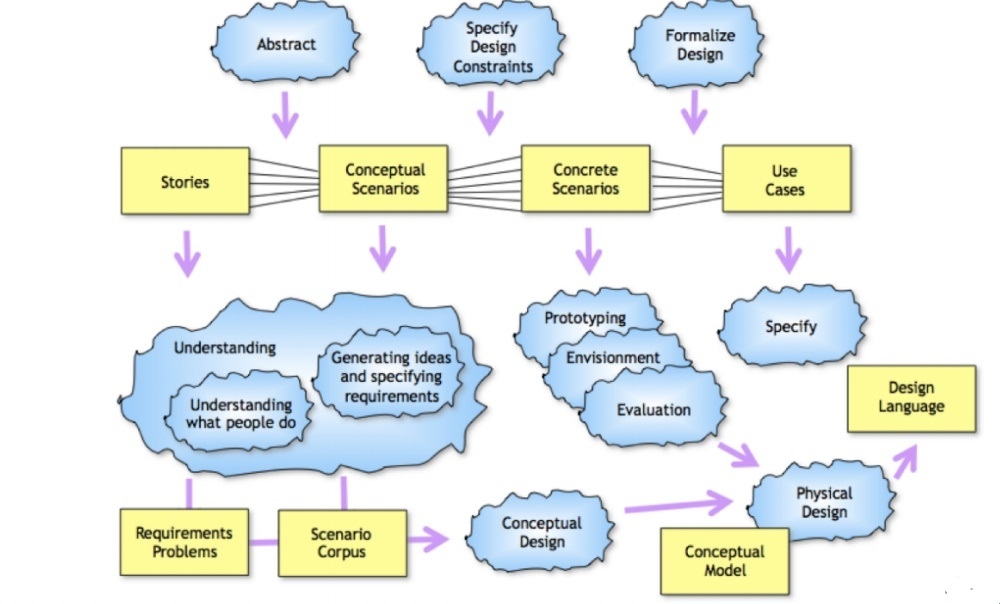
\includegraphics[width=1\textwidth]{Grafik/scenarioModel}
	\caption{Scenario-based Design Method.}
	\label{scenarioModel}
\end{figure}